\section{How do the different layers of a CNN train over time? How much pre-training is sufficient?}
\label{sec:speed}
Pre-Training is the process of initializing CNN parameters for a target application using images from a (generally larger) separate dataset. Features learned by a CNN pre-trained on Imagenet have been shown to generalize and achieve state of art results across multiple computer vision datasets (see section \ref{sec:fine} and \cite{Decaf}). Since, no single image dataset fully captures the variation in natural images, all datasets are biased (cite Alyosha). Consequently, it can be expected that excessive pre-training can cause the CNN to overfit on Imagenet and thus hurt generalization performance. 

In order to determine if this is indeed the case, we analysed the performance of features extracted  at various time steps from a network trained on Imagenet for classifying images on the PASCAL-2007 dataset. Linear SVMs were trained for classification and the results are presented in table \ref{table:det-traj-classify}. It is quite surprising to note that by 15K iterations all layers are within 80\% and at 50K iterations within 90\% of there final performance. This strongly indicates that a great portion of training required for generalization happens quite quickly. 


\setlength{\tabcolsep}{4pt}
\begin{table}[t!]
\begin{center}
\caption{Variation in classification accuracy (mean-AP) on PASCAL-2007 challenge using features extracted from different layers of Alex-Net as a function of number of iterations.}
\label{table:det-traj-classify}
\begin{tabular}{lcccccccc}
\hline\noalign{\smallskip}
Layer  & 5K & 15K & 25K & 35K & 45K & 95K & 105K & 310K \\
\noalign{\smallskip}
\hline
\noalign{\smallskip}
conv-1 & 23.0 & 24.3 & 24.4 & 24.5 & 24.6 & 24.8 & 24.7 & 25.1\\
conv-2 & 33.7 & 40.4 & 40.9 & 41.8 & 42.0 & 43.2 & 44.0 & 45.0\\
conv-3 & 34.2 & 46.8 & 47.0 & 48.2 & 48.5 & 49.4 & 51.6 & 50.1\\
conv-4 & 33.5 & 49.0 & 48.7 & 50.2 & 50.6 & 51.6 & 54.1 & 54.2\\
conv-5 & 33.0 & 53.4 & 55.0 & 56.8 & 57.4 & 59.2 & 63.5 & 65.6\\
fc-6 & 34.2 & 59.7 & 62.6 & 62.7 & 64.1 & 65.6 & 69.3 & 70.6\\
fc-7 & 30.9 & 61.3 & 64.1 & 65.1 & 65.8 & 67.8 & 71.8 & 73.2\\
\hline
\end{tabular}
\end{center}
\end{table}
\setlength{\tabcolsep}{1.4pt}

\begin{figure}[t!]
\centering
\subfloat[5K Iterations]{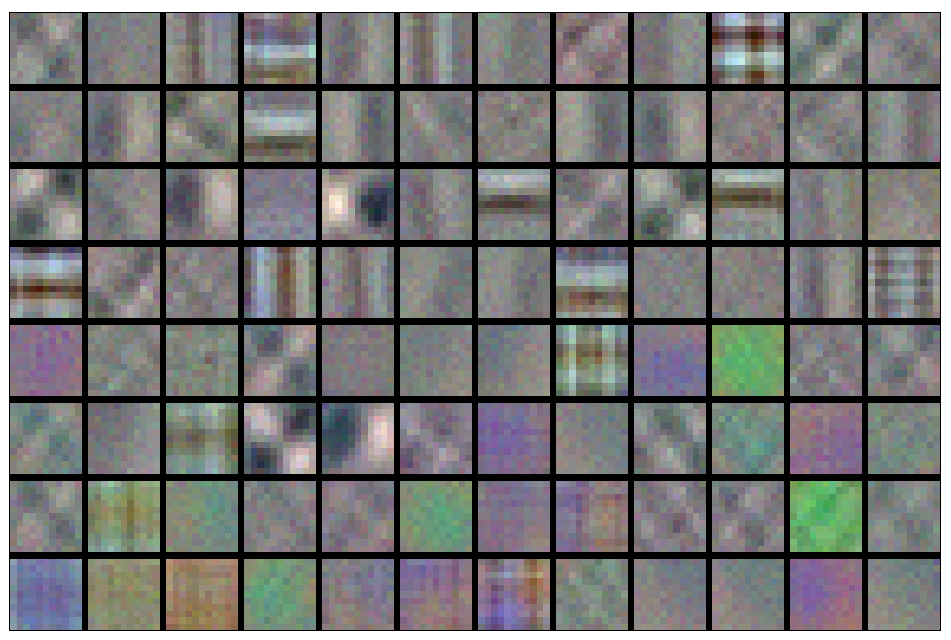
\includegraphics[scale=0.10]{images/l1_filters_iter5000.png}} \hspace{2mm}
\subfloat[15K Iterations]{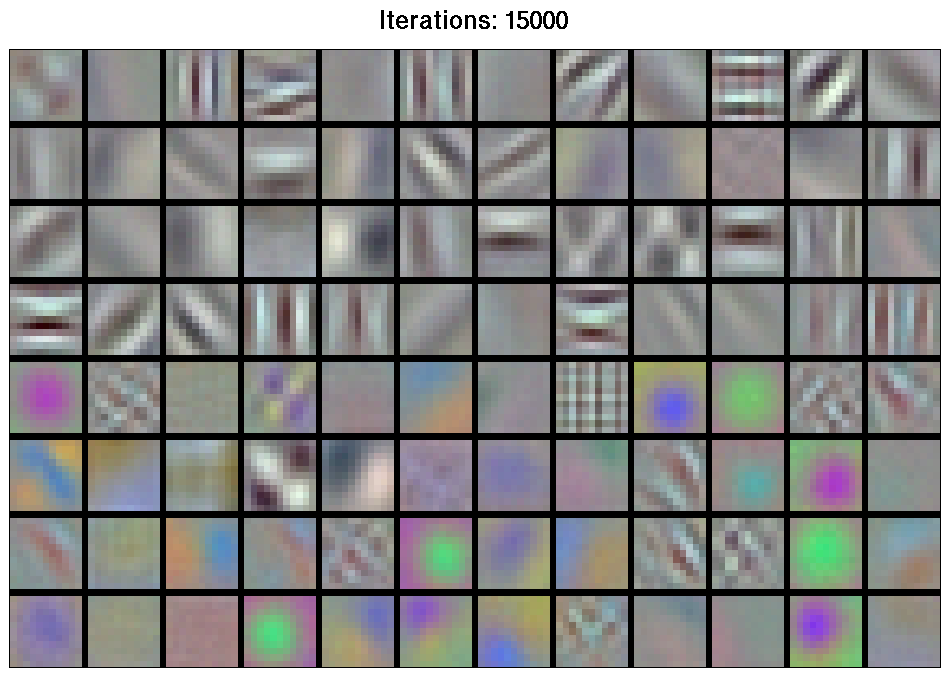
\includegraphics[scale=0.10]{images/l1_filters_iter15000.png}} \hspace{2mm}
\subfloat[225K Iterations]{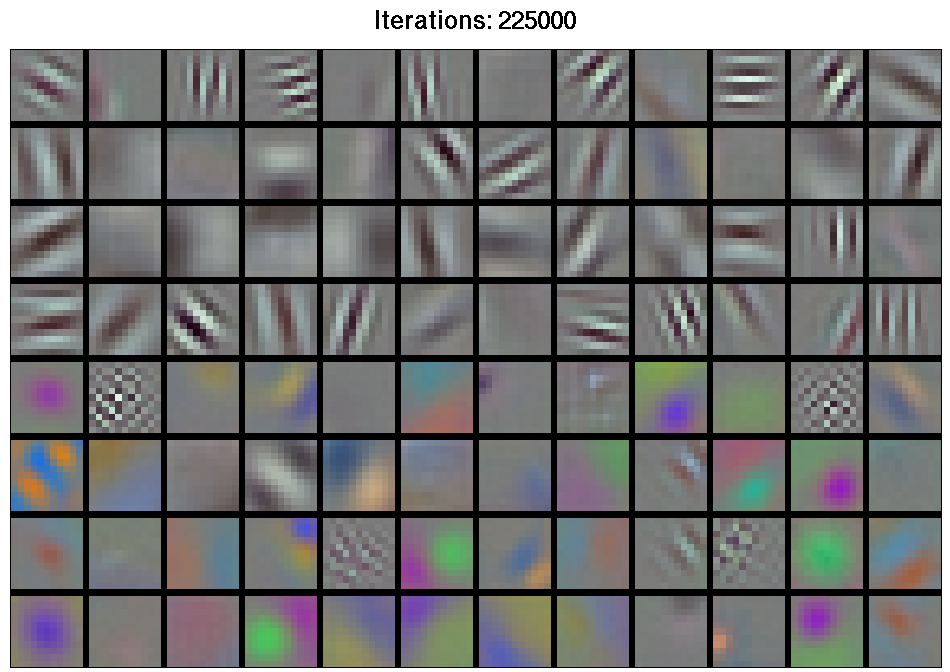
\includegraphics[scale=0.10]{images/l1_filters_iter225000.png}}
\caption{(a),(b),(c) show conv-1 filters after 5K, 15K and 225K iterations of training respectively. One pass (epoch) over the entire Imagenet-ILSVRC12 dataset takes approximately 5K iterations. Notice, that just after 15K iterations these filters closely resemble their final state.}
\label{fig:conv1}
\end{figure}


** To Come .. pending results **

\setlength{\tabcolsep}{1pt}
\begin{table}[t!]
\begin{center}
\caption{Performance of 50-50 network for detection on pascal-voc-2007 challenge. (l5 is conv-5 and l7 is fc-7)}
\label{table:det-trajectory}
\scalebox{1.00}{
\begin{tabular}{|l|cccc|}
\hline
 & 50K & 105K & 205K & 305K \\
\hline
det & - & - & - & - \\
sun-397 & - & - & - & - \\
\hline
\end{tabular}}
\end{center}
\end{table}
\setlength{\tabcolsep}{1.4pt}
The above analysis reinforces our belief that indeed majority of training required for generalization happens quite quickly as compared to the full training time of the network. This observation suggest that there may exist clever ways which can help us speed up the training.

